\documentclass[a4paper]{article}

\usepackage[utf8]{inputenc}

\usepackage{url}
\usepackage[hidelinks]{hyperref}

\usepackage{caption}

\usepackage{listings}

\usepackage{color}

% *** GRAPHICS RELATED PACKAGES ***
%\usepackage[pdftex]{graphicx}
\usepackage{graphicx}
%\usepackage[dvips]{graphicx}
% to place figures on a fixed position
\usepackage{float}

\usepackage[margin=1in]{geometry}

\title{OpenFlow \& Mininet – template}
\author{}
\date{}


\begin{document}

\maketitle

\tableofcontents

\section{Introduction}
As computers have become more popular, they have required to be interconnected in order to communicate with each other. The Internet is a network of autonomous systems (AS) and each AS is a collection of IP networks. Therefore, the Internet is often called 'the network of networks'. Between autonomous systems, inter-domain routing is used (BGP in this lab, which is standard for Internet routing), whereas in the AS, intra-domain routing is applied (the widely used OSPF in this lab). Soon, we will see the interaction of these protocols. The goal of this lab is to show the complexity of Internet and to present its routing solutions using a simplified model. Please note that the Internet topology and the number of connections are unknown. There are only approximate data about how billions of hosts are connected to the global network.

\section{Internet routing}

\subsection{Routing protocol operations; routing table, forwarding table}

In order to have a functional IP routing, each node must have a forwarding table which contains IP prefixes and the associated next hop addresses. Forwarding table is sometimes called routing table but it can be misleading and it is important to distinguish these terms. When we send a packet to a destination address, the network layer needs to make a lookup in the forwarding table. Then the packet is sent to the corresponding IP address. The forwarding table can be created either manually or by using dynamic routing protocols. A single device may run multiple routing protocols. These protocols propose changes to the forwarding table but the final decision is made by the network layer of the device (for instance, the operating system). Each routing process has a separate table which is used to make a suggestion, also known as the routing table. Although routing processes run on the same device, they don't communicate with each other by default. As a result, one process doesn't know about routes that other processes have found. However, we can tell them to exchange routing information and to propagate routes (redistribution). Thus, route redistribution allows routes from one routing protocol to be advertised into another routing protocol (but it doesn't mean that each protocol makes the same suggestion to modify the forwarding table). In some cases, redistribution is not recommended. For example, if a protocol that uses a huge global database injected a large number of routes into a less scalable interior gateway protocol (IGP), the IGP would be overwhelmed and the routing process would fail.

\subsection{BGP}

Nowadays the Border Gateway Protocol is used on the Internet. BGP is a path-vector routing protocol. It differs from the distance vector (RIP, EIGRP) and link-state (OSPF) protocols. A BGP routing table entry includes the destination network (prefix), next-hop address and the path to reach the destination host. When an AS boundary router (ASBR) that uses BGP receives a path-vector message from an other ASBR, it needs to check the advertised route against its policy. If the local policy allows the route, the router sends a modified path-vector message to its neighbor: it adds its own AS number and path information to the message.
BGP was designed to replace Exterior Gateway Protocol (EGP). Due to its hierarchical architecture, EGP can't handle the routing in modern networks. However, BGP provides distributed operation. It have had many versions since 1994, but the major enhancement was the support for Classless Inter-Domain Routing (CIDR) and use of route aggregation to decrease the size of routing tables. Introducing CIDR was inevitable to help slow the rapid exhaustion of IPv4 addresses. Using CIDR, the division point between the subnet/network ID and the host ID can be on any address bit boundary, instead of on 8-bit segments. Route aggregation reduces the number of entries in the routing table. Aggregation makes it possible to advertise many subnets as a single, larger network (supernet). For example, the summary address of 37.0.1.0/24, 37.0.2.0/24...37.0.255.0/24 networks is 37.0.0.0/16. BGP is required of most Internet service providers (ISPs) to establish routing between one another.


\subsection{BGP operation}

BGP neighbors are established by manual configuration between routers to create a TCP session on port 179. A BGP speaker sends 19-byte keep-alive messages every 60 seconds to maintain the connection. Among routing protocols, BGP is unique in using TCP as its transport protocol and also in manual neighbor configuration. In case of interior gateway protocols, routers become neighbors automatically if possible, whereas BGP requires to configure the neighbor using its IP address. BGP can be used between different autonomous systems and also between two routers in the same AS. When BGP runs between two peers in the same AS, it is referred to as Internal BGP (iBGP or Interior Border Gateway Protocol). When it runs between different autonomous systems, it is called External BGP (eBGP or Exterior Border Gateway Protocol). Routers on the boundary of one AS exchanging information with another AS are called border or edge routers or eBGP peers. Please note that IGP and eBGP routes take precedence over iBGP. BGP has optional capabilities including multiprotocol extensions and various recovery modes. These capablilities can be negotiated during the peering handshake, when OPEN messages are exchanged. In order to make decisions in its operations with peers, a BGP peer uses a finite state machine (FSM) that consists of six states. The FSM is shown in Figure~\ref{fig:BGP-FSB}.

\begin{figure}[H]
    \centering
    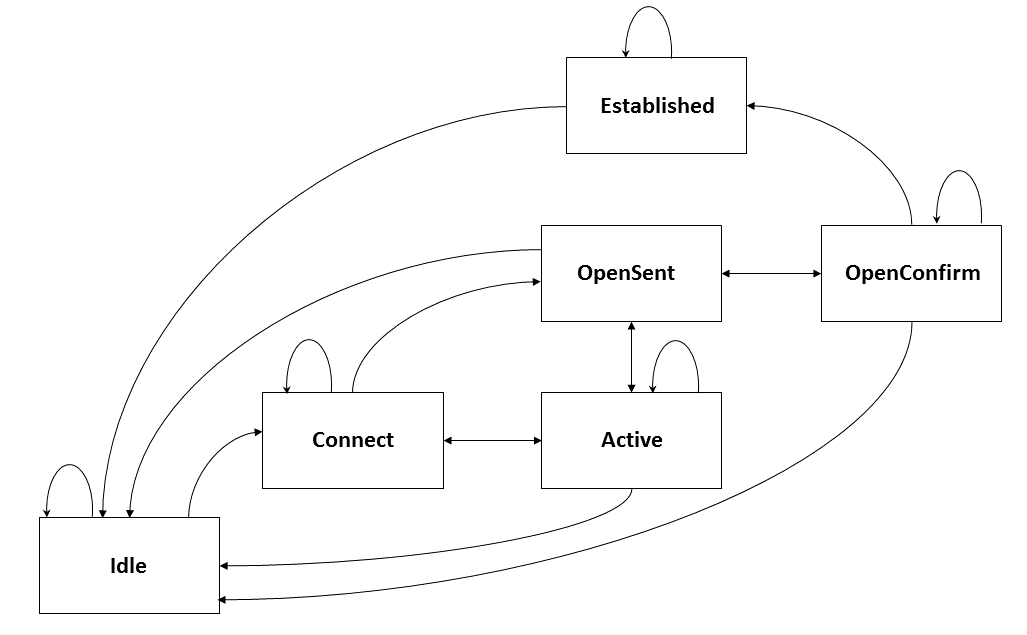
\includegraphics[width=0.9\textwidth]{figures/bgp-fsm.png}
    \caption{BGP neighbouring session establishment state transition diagram}
    \label{fig:BGP-FSM}
\end{figure}

The first state is the "Idle" state. In the "Idle" state, BGP waits for connection attempts from neighbors, initializes all resources and initiates a TCP connection to the peer. The second state is "Connect". In the "Connect" state, the router waits for the TCP connection to complete and transitions to the "OpenSent" state if successful. Normally, BGP does not spend much time in this state. If unsuccessful, it starts a timer and transitions to the "Active" state upon expiration. In the "Active" state, the router resets the timer to zero and returns to the "Connect" state. If connection attempts fail many times, it transitions back to "Idle" state. In the "OpenSent" state, the router sends an Open message and waits for one in return. Once the message has been received, the router checks the validity of the Open message. If there is no error, a Keepalive message is sent, various timers are set and the state is changed to OpenConfirm. If there is an error, the router sends a Notification message to the peer indicating why the error occurred. In the "OpenConfirm" state, the peer is listening for a Keepalive message from its peer. If a Keepalive message is received and no timer has expired before reception of the Keepalive, BGP transitions to the "Established" state. If a timer expires before a Keepalive message is received, or if an error condition occurs, the router transitions back to the Idle state. In the "Established" state, the router can send/receive Keepalive, Update and Notification messages to/from its peer. If there is any error, BGP transitions back to the "Idle" state. The Update messages contain information about each route being advertised to the BGP peer. According to the BGP terminology, a basic CIDR route description is called Network Layer Reachability Information (NRLI). NLRI consists of destination network prefix, subnet mask, AS path and next-hop address.
All routers within a single AS and participating in BGP routing must be configured in a full mesh: each router must be configured as peer to every other router. This causes scaling problems, since the number of required connections grows quadratically with the number of routers involved. To reduce the problem, BGP implements additional options in complex networks. 
A given BGP router may accept NLRI Updates from and advertise to multiple neighbors. BGP maintains its own routing table, called the Local Routing Information Base (Loc-RIB), separate from the main routing table of the router. For each neighbor, the BGP process maintains an Adjacent Routing Information Base, Incoming (Adj-RIB-In) containing the NLRI received from the neighbor, and an Adj-RIB-Out (Outgoing) for NLRI to be sent to the neighbor.
The BGP standard specifies a number of decision factors for selecting NLRI to go into the Loc-RIB. This is more than the ones that are used by any other common routing process. The first decision point for evaluating NLRI is that its next-hop attribute must be reachable, so there must be an active route already in the main routing table of the router. Next, for each neighbor, the BGP process applies various criteria to decide which routes should go into the Adj-RIB. Only one route to each destination will be installed in the Adj-RIB. This process will also delete any routes from the Adj-RIB that are withdrawn by the neighbor.
Whenever an Adj-RIB changes, the main BGP process decides if any of the neighbor's new routes are preferred to routes already in the Loc-RIB. If so, it replaces them. If a given route is withdrawn by a neighbor, and there is no other route to that destination, the route is removed from the Loc-RIB. 
In summary: at the beginning, NLRIs are received and added to the Adj-RIB. After evaluating priorities and policies, NLRIs go into the Loc-RIB. BGP advertises the Loc-RIB to the main routing table manager which creates the router's forwarding table.


\section{Router implementation}

\subsection{Cisco IOS}

Cisco IOS is a family of software used on most Cisco routers and network switches. IOS is a package of routing, switching, internetworking and telecommunications functions integrated into a multitasking operating system. The IOS command line interface provides a fixed set of multiple-word commands. The set available is determined by the "mode" and the privilege level of the current user. "Global configuration mode" provides commands to change the system's configuration, and "interface configuration mode" provides commands to change the configuration of a specific interface. All commands are assigned a privilege level from 0 to 15, and can only be accessed by users with the necessary privilege. Through the CLI, the commands available to each privilege level can be defined.
The required commands for this lab can be found in Section~\ref{sec:Cisco-guide} guide.

\subsection{Quagga}
In addition to network device manufacturers, there is an open-source software suite for Linux (Quagga) that implements dynamic routing protocols. A system with Quagga installed acts as a dedicated router. Quagga supports the most common IPv4 routing protocols (RIP, OSPF, BGP) and IPv6 protocols as well. The CLI commands are similar to the ones in Cisco IOS. Routing protocol implementations run in separate daemon processes:
\begin{itemize}
    \item OSPF protocol: ospfd (port:2604)
    \item BGP protocol: bgpd (port: 2605)
    \item RIP (ripd), IS-IS (isisd), etc.
\end{itemize}

When a Quagga daemon process starts, it automatically generates the required configuration files:

\begin{itemize}
    \item /etc/quagga/zebra
    \item /etc/quagga/bgpd.conf
\end{itemize}

We can use the vtysh command to access the dedicated Quagga terminal emulator. In order to login and change configuration, the enable command have to be entered which requires a password. Like on Cisco devices, you can type as few characters as are needed to make the command unique. Command line completion can also be used by pressing the TAB key. If you press TAB a second time, possible completions will be recommended. Typing '?' will list the available commands with a description.
Some useful Quagga commands:

\begin{itemize}
\item Switching to configuration mode: configure terminal (conf t)
\item Configuring a given ethX interface: interface ethX
\item Setting an IP address: ip address <address/prefix-length>
\item Changing interface state to UP: no shutdown (it's done automatically in Quagga, required if using Cisco IOS)
\item Leaving (interface) config mode: exit
\item Displaying current config: write terminal
\item Saving config: copy running-config startup-config (copy run start)
\item Configuring routing protocol: router bgp \textless~AS_number~\textgreater
\end{itemize}

Some useful Linux commands:

\begin{itemize}
\item Assigning IP address to an interface: ip address add \textless~ip-address~\textgreater/~\textless~netmask~\textgreater dev ethX
\item Enabling interface: ip link set ethX up
\item Default gateway: ip route add 0.0.0.0/0 via \textless~ip-address~\textgreater
\end{itemize}

An example intro on Quagga can be found here
Detailed Quagga documentation can be found here: \url{http://downloads.pf.itd.nrl.navy.mil/docs/ospf-manet/quagga.pdf}

\subsubsection{Further Reading on Quagga}

\begin{itemize}
    \item \href{http://unixlinux.tmit.bme.hu/Quagga}{TMIT BME Intro to Quagga}
    \item \href{http://downloads.pf.itd.nrl.navy.mil/docs/ospf-manet/quagga.pdf}{Detailed Quagga documentation}
\end{itemize}


\appendix

\section{Entry quiz sample questions}

\begin{enumerate}
    \item Describe briefly the main concept of the OpenFlow recommendation.
    \item What are the components of an OpenFlow network?
\end{enumerate}

\section{Lab exercises}

\subsection{Lab environment}

\end{document}